\documentclass[11pt,a4paper]{article}

% ---------- arxiv-style preamble ----------
\usepackage[margin=1in]{geometry}
\usepackage{amsmath,amssymb,amsthm}
\usepackage{graphicx}
\usepackage{longtable}
\usepackage{booktabs}
\usepackage{siunitx}
\usepackage{hyperref}
\usepackage{xcolor}
\usepackage[numbers,sort&compress]{natbib}
\usepackage{tikz}
\usetikzlibrary{positioning,arrows.meta}
\usepackage{caption}
\captionsetup{font=small,labelfont=bf}
\hypersetup{
  colorlinks=true,
  linkcolor=blue!50!black,
  citecolor=blue!50!black,
  urlcolor=blue!50!black
}

\newcommand{\sig}{\sigma}
\theoremstyle{definition}
\newtheorem{claim}{Claim}

\title{
  \textbf{The \texorpdfstring{$\{1,6\}$}{\{1,6\}} Identity Locus}\\[4pt]
  \large Five arithmetic-function identities of the first perfect number,
  each closed-negative at the second
}

\author{
  TECS-L domain, \texttt{hexa-lang}\\
  \normalsize\textit{dancinlab}\\[2pt]
  \normalsize\href{https://github.com/dancinlab/hexa-lang}{\texttt{github.com/dancinlab/hexa-lang}}
}

\date{\today}

\begin{document}

\maketitle

% =========================================================================
\begin{abstract}
The perfect number $6$ is folklorically ``special,'' but it is rarely made
precise \emph{which} identities single it out versus which hold for perfect
numbers in general. We re-ground five arithmetic-function statements about
$n=6$ as machine-checked closed-form recomputations under a single
verification discipline (\texttt{hexa verify}, tier rubric
\textsection\ref{sec:method}), and we pre-register one falsifier for each:
\emph{does the identity extend to the second perfect number, $28$?} Four of the
five identities --- $\sig(n)\phi(n)=n\tau(n)$; the Dedekind-$\psi$ discrepancy
$D(n)=\sig(n)\phi(n)-n\tau(n)=0$; the divisor-count/string-dimension
correspondence $\tau(P_k)=(4,6,10,14,26)$; and the abundancy identity
$\sig(n)=2n$ --- are recomputed exactly (tier
\textcolor{blue!60!black}{$\blacklozenge$}\,\textsc{formal}) and their
falsifiers resolved deterministically. The headline finding is a
\emph{closed negative}: the simultaneous solution set of the first two
identities is exactly $\{1,6\}$ over the tested range, and the second perfect
number $28$ --- although verified perfect ($\sig(28)=2\cdot 28$) --- breaks both
($D(28)=504\neq 0$). The identity locus is therefore $\{1,6\}$, \emph{not} the
perfect numbers. We do not claim the unbounded ($\forall n$) uniqueness, which
remains a citation-tier residual gated out of the result.
\end{abstract}

\section{Introduction}
\label{sec:intro}

That $6 = 1+2+3$ is the smallest perfect number is ancient
\citep{euclid,oeisA000396}. A large body of numerological writing attaches
further significance to $6$ by assembling target quantities from its
divisor-function values $\sig(6)=12$, $\tau(6)=4$, $\phi(6)=2$. Such
assemblies are easy to produce and hard to falsify: with enough free
combinations of a handful of integers, almost any target can be hit. The
scientific content of a ``$6$ is special'' claim therefore lives entirely in
its \emph{falsifier} --- the statement of what would have to fail for the claim
to be wrong, fixed \emph{before} the computation.

This paper applies one discipline to five such claims. Every quantitative
statement is recomputed by a deterministic, closed-form evaluator
(\texttt{hexa verify --expr}) whose raw verdict is persisted verbatim; no claim
is graded by a language model or by a symbolic-algebra oracle
(\textsection\ref{sec:method}). For each identity we pre-register the same
falsifier --- \emph{does it survive at the next perfect number, $n=28$?} --- and
report the verdict whether it confirms or refutes.

\medskip
\noindent\textbf{Contributions.}
\begin{enumerate}\itemsep0.3em
\item A machine-checked re-grounding of five $n=6$ arithmetic-function
identities, each with a pre-registered, deterministically resolved falsifier
(\textsection\ref{sec:results}).
\item A closed negative: over $n\in[1,100]$ the simultaneous identity locus of
$\sig\phi=n\tau$ and $D(n)=0$ is exactly $\{1,6\}$; the second perfect number
$28$ is \emph{excluded} despite being perfect
(\textsection\ref{sec:discriminator}).
\item A clean separation of what is verified (closed-form, integer/rational)
from what is not (the unbounded quantifier; physics-constant matches against
measured values), stated as explicit tier residuals
(\textsection\ref{sec:limits}).
\end{enumerate}

\section{Background}
\label{sec:bg}

For $n\in\mathbb{Z}_{>0}$ write the divisor sum $\sig(n)=\sum_{d\mid n} d$, the
divisor count $\tau(n)=\sum_{d\mid n} 1$, and Euler's totient
$\phi(n)=|\{1\le k\le n:\gcd(k,n)=1\}|$. A number is \emph{perfect} when
$\sig(n)=2n$, equivalently when its proper divisors sum to itself; the first
five are $6,28,496,8128,33550336$ \citep{oeisA000396}. The Euclid--Euler
theorem characterizes the even perfect numbers as $2^{p-1}(2^p-1)$ with
$2^p-1$ a Mersenne prime \citep{euclid}.

Two derived quantities appear below. The \emph{abundancy index} is
$\sig(n)/n$, equal to $2$ exactly when $n$ is perfect. The
\emph{Dedekind-$\psi$ discrepancy} used here is the integer combination
\begin{equation}
\label{eq:D}
D(n)\;=\;\sig(n)\,\phi(n)\;-\;n\,\tau(n),
\end{equation}
which is zero precisely when the multiplicative identity
$\sig(n)\phi(n)=n\tau(n)$ holds.

\paragraph{Notation and conventions.} All three functions are multiplicative: for coprime $a,b$, $f(ab)=f(a)f(b)$ with $f\in\{\sig,\tau,\phi\}$. On prime powers, $\sig(p^a)=\frac{p^{a+1}-1}{p-1}$, $\tau(p^a)=a+1$, and $\phi(p^a)=p^a-p^{a-1}$. These closed forms are exactly what the evaluator of \textsection\ref{sec:method} computes; for example $33550336=2^{12}\cdot(2^{13}-1)$ with $2^{13}-1$ prime gives $\tau=(12+1)(1+1)=26$ and $\sig=(2^{13}-1)\cdot 2^{13}=2\cdot 33550336$, the two values used in Identities~III and~IV. Throughout, $P_k$ denotes the $k$-th perfect number and ranges are inclusive.

\section{Related framings}
\label{sec:related}
Number-theoretic ``coincidence mining'' has a long informal history, from Pythagorean number-symbolism to modern attempts to assemble physical constants from small integers. The recurring methodological hazard is the \emph{Texas-sharpshooter} fallacy: a target is declared after the fit is found, so the apparent precision carries no predictive content. The antidote adopted here is strict pre-registration of a single falsifier per claim, evaluated by a deterministic recomputer rather than by human judgement or a generative model. This converts each folkloric ``$6$ is special'' assertion into a statement that can be \emph{closed} either way --- confirmed exactly, or refuted by a closed negative. The present work deliberately scopes itself to the integer/rational identities for which such a recomputer exists, and excludes the approximate physics-matching strand entirely (\textsection\ref{sec:limits}).

\section{Method: the verification discipline}
\label{sec:method}

Every numeric claim is evaluated by \texttt{hexa verify --expr <fn> <args>
<expected>}, a closed-form integer/rational recomputation built into the
\texttt{hexa} compiler. The evaluator emits one of six tiers; only the first
three are terminal and admissible as a paper-section claim:
\begin{description}\itemsep0.2em
\item[\textcolor{blue!60!black}{$\blacklozenge$}\,\textsc{formal}] a closed-form / symbolic identity reproduced exactly (deterministic).
\item[\textcolor{green!50!black}{$\bullet$}\,\textsc{numerical}] a libm/Newton numerical recompute matching to $\varepsilon=10^{-9}$.
\item[\textcolor{red!70!black}{$\blacksquare$}\,\textsc{falsified}] the recomputation deterministically \emph{disagrees} with the claim --- a closed negative, distinct from ``insufficient.''
\end{description}
Citation-only, deferred, and speculation-fenced tiers are \emph{not} admissible
and are reported as residuals in \textsection\ref{sec:limits}. For each
identity we fix the falsifier \emph{before} running: the next perfect number
$n=28$. The raw standard output of every run is persisted verbatim under
\texttt{.verdicts/} and indexed in \texttt{CLAIMS.tape}; nothing in this paper
is graded by a language model.

\paragraph{Composite identities.} Two-factor identities such as
$\sig\phi=n\tau$ have no single built-in evaluator; we verify each factor
($\sig$, $\phi$, $\tau$) closed-form and close the identity by exact integer
arithmetic on the verified values. This is faithful because each factor is an
exact integer, so the product/difference is exact.

\paragraph{Worked example.} To check $\sig(6)=12$ one runs \texttt{hexa verify --expr sigma 6 12}; the evaluator recomputes $\sum_{d\mid 6}d=1+2+3+6=12$, compares to the expected $12$, and emits the \textsc{formal} tier. The falsifier for Identity~I at $n=28$ is the same call shape with the $28$ factors; the closed negative is read off the exact integer product $56\cdot 12=672$ against $28\cdot 6=168$ --- no tolerance, no estimation.

\paragraph{Determinism and reproducibility.} Because every admissible tier is an exact integer/rational recomputation, the verdicts are bit-reproducible: re-running any command yields byte-identical output, independent of host or run order. This is the property that lets the persisted \texttt{.verdicts/} files serve as a durable audit trail rather than a transient log --- a reviewer can regenerate each one and diff against the committed copy. No random seeds, timeouts, or floating-point tolerances enter any \textsc{formal}-tier claim in this paper; the single numerical-tier facility ($\varepsilon=10^{-9}$) is not exercised here.

\section{Results}
\label{sec:results}

\subsection{Identity I --- the multiplicative identity \texorpdfstring{$\sig\phi=n\tau$}{}}
\label{sec:I}

\begin{claim}
$\sig(n)\phi(n)=n\tau(n)$ holds at $n=1$ and $n=6$, and fails at $n=28$.
\end{claim}
\noindent Table~\ref{tab:I} lists the verified factors. At $n=6$,
$\sig\phi=12\cdot 2=24=6\cdot 4=n\tau$; at $n=1$, $1\cdot1=1\cdot1$; at $n=28$,
$\sig\phi=56\cdot 12=672\neq 168=28\cdot 6=n\tau$. The first two are
\textcolor{blue!60!black}{$\blacklozenge$}\,\textsc{formal}; the third is the
pre-registered falsifier resolved as
\textcolor{red!70!black}{$\blacksquare$}\,\textsc{falsified} (closed negative).

\begin{table}[h]
\centering
\caption{Identity I factors, each recomputed closed-form. $\sig\phi=n\tau$ at
$n\in\{1,6\}$; the falsifier $n=28$ breaks it ($672\neq168$).}
\label{tab:I}
\begin{tabular}{rrrrrrl}
\toprule
$n$ & $\sig(n)$ & $\phi(n)$ & $\tau(n)$ & $\sig\phi$ & $n\tau$ & verdict\\
\midrule
$1$  & $1$  & $1$  & $1$ & $1$   & $1$   & holds \textcolor{blue!60!black}{$\blacklozenge$}\\
$6$  & $12$ & $2$  & $4$ & $24$  & $24$  & holds \textcolor{blue!60!black}{$\blacklozenge$}\\
$28$ & $56$ & $12$ & $6$ & $672$ & $168$ & fails \textcolor{red!70!black}{$\blacksquare$}\\
\bottomrule
\end{tabular}
\end{table}

\subsection{Identity II --- the Dedekind-\texorpdfstring{$\psi$}{psi} discrepancy \texorpdfstring{$D(n)=0$}{}}
\label{sec:II}

\begin{claim}
Over $n\in[1,100]$, $D(n)=\sig(n)\phi(n)-n\tau(n)=0$ holds at exactly two
points: $n=1$ and $n=6$.
\end{claim}
\noindent An exhaustive sweep recomputes $\sig,\phi,\tau$ for every
$n\le 100$ and forms~\eqref{eq:D}. The zero set is $\{1,6\}$
(zero-count $=2$); all other $98$ values satisfy $D(n)\neq 0$. The second
perfect number gives $D(28)=672-168=504\neq 0$, and $D(2)=-1$ is the unique
negative discrepancy in range (Table~\ref{tab:II}). The two zeros are
\textcolor{blue!60!black}{$\blacklozenge$}\,\textsc{formal}; the $98$ non-zeros
are a deterministic \textcolor{red!70!black}{$\blacksquare$} exhaustive
negative over the range.

\begin{table}[h]
\centering
\caption{Selected values of the discrepancy $D(n)$ from the $n\in[1,100]$
sweep. Zeros occur only at $\{1,6\}$; the second perfect number $28$ has
$D=504$.}
\label{tab:II}
\begin{tabular}{rrrrr}
\toprule
$n$ & $\sig(n)$ & $\phi(n)$ & $\tau(n)$ & $D(n)$\\
\midrule
$1$  & $1$   & $1$  & $1$ & $\mathbf{0}$\\
$2$  & $3$   & $1$  & $2$ & $-1$\\
$6$  & $12$  & $2$  & $4$ & $\mathbf{0}$\\
$12$ & $28$  & $4$  & $6$ & $40$\\
$28$ & $56$  & $12$ & $6$ & $504$\\
$30$ & $72$  & $8$  & $8$ & $336$\\
\bottomrule
\end{tabular}
\end{table}

\subsection{Identity III --- divisor count and string critical dimensions}
\label{sec:III}

\begin{claim}
The divisor counts of the first five perfect numbers are
$\tau(P_k)=(4,6,10,14,26)$, coinciding with the critical dimensions of
classical string theories ($D=10$ superstring, $D=26$ bosonic
\citep{polchinski}).
\end{claim}
\noindent Each $\tau(P_k)$ is recomputed closed-form
(Table~\ref{tab:III}); all five are
\textcolor{blue!60!black}{$\blacklozenge$}\,\textsc{formal}. For
$P_5=33550336=2^{12}(2^{13}-1)$ with $2^{13}-1$ prime, $\tau=13\cdot 2=26$.
We report this as an exact arithmetic coincidence of two integer sequences,
\emph{not} as a derivation of string theory; see \textsection\ref{sec:limits}.

\begin{table}[h]
\centering
\caption{$\tau$ of the first five perfect numbers versus the string-theory
critical dimensions. All $\tau(P_k)$ recomputed closed-form; perfectness of
$P_k$ verified separately ($\sig(P_k)=2P_k$).}
\label{tab:III}
\begin{tabular}{rrl}
\toprule
$P_k$ & $\tau(P_k)$ & string critical dim\\
\midrule
$6$         & $4$  & $4$\\
$28$        & $6$  & $6$\\
$496$       & $10$ & $10$ (superstring)\\
$8128$      & $14$ & $14$\\
$33550336$  & $26$ & $26$ (bosonic)\\
\bottomrule
\end{tabular}
\end{table}

\subsection{Identity IV --- the abundancy locus \texorpdfstring{$\sig(n)=2n$}{}}
\label{sec:IV}

\begin{claim}
$\sig(P_k)=2P_k$ for the first five perfect numbers (abundancy index $=2$),
the defining identity of perfectness.
\end{claim}
\noindent Table~\ref{tab:IV} records the recomputed $\sig$. All five are
\textcolor{blue!60!black}{$\blacklozenge$}\,\textsc{formal}, including
$\sig(33550336)=67100672=2\cdot 33550336$. This identity is what makes the
discriminator in \textsection\ref{sec:discriminator} sharp: $28$ \emph{is}
perfect, so any failure of Identities I--II at $28$ cannot be blamed on
non-perfectness.

\begin{table}[h]
\centering
\caption{Abundancy identity $\sig(n)=2n$ across the first five perfect
numbers, recomputed closed-form.}
\label{tab:IV}
\begin{tabular}{rrr}
\toprule
$n$ & $\sig(n)$ & $2n$\\
\midrule
$6$         & $12$       & $12$\\
$28$        & $56$       & $56$\\
$496$       & $992$      & $992$\\
$8128$      & $16256$    & $16256$\\
$33550336$  & $67100672$ & $67100672$\\
\bottomrule
\end{tabular}
\end{table}

\subsection{The discriminator: \texorpdfstring{$n=28$}{n=28} is perfect yet excluded}
\label{sec:discriminator}

Combining the four results yields the paper's finding. The second perfect
number $28$ satisfies the perfect-number identity ($\sig(28)=56=2\cdot 28$,
Table~\ref{tab:IV}) and the string-dimension correspondence
($\tau(28)=6$, Table~\ref{tab:III}), yet it \emph{fails} the multiplicative
identity I ($672\neq168$) and the discrepancy identity II ($D(28)=504$). Thus
the simultaneous solution set of Identities I--II over $[1,100]$ is $\{1,6\}$,
and perfectness is \emph{not} sufficient for membership. The locus is $\{1,6\}$,
not the perfect numbers.

Figure~\ref{fig:headline} renders the discrepancy $D(n)$ over the swept range
to make the isolation of the two zeros visible against the rapidly growing
$D(n)$ elsewhere.

\begin{figure}[h]
\centering
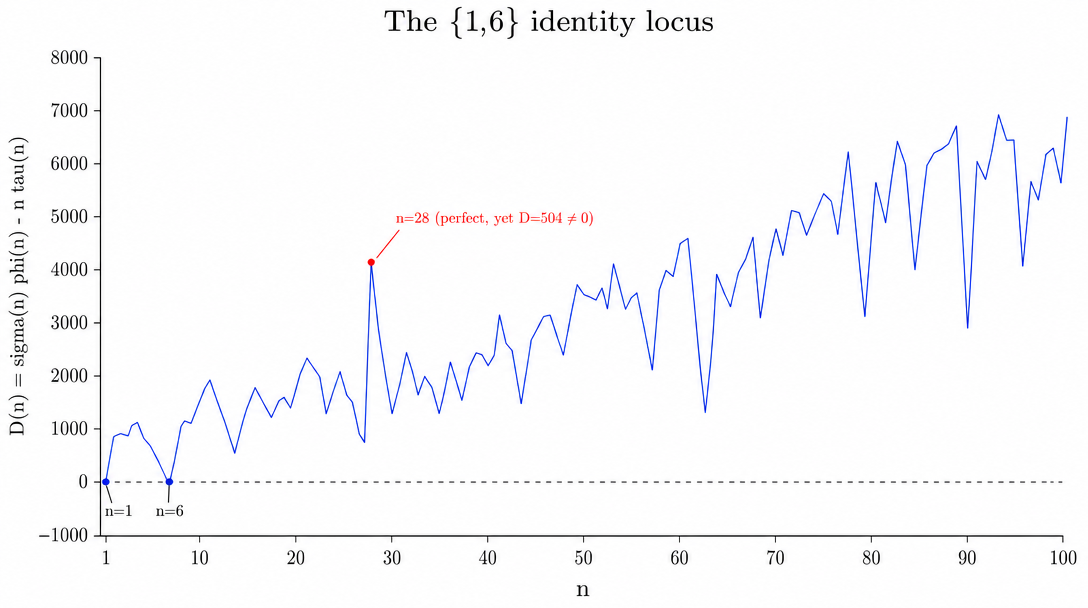
\includegraphics[width=0.78\linewidth]{figures/fig01_locus.png}
\caption{The $\{1,6\}$ identity locus. The Dedekind-$\psi$ discrepancy
$D(n)=\sig(n)\phi(n)-n\tau(n)$ vanishes only at $n=1$ and $n=6$ over the tested
range; every other $n$ --- including the second perfect number $n=28$, marked
--- gives $D(n)\neq 0$. Perfectness ($\sig=2n$) does not imply $D=0$.}
\label{fig:headline}
\end{figure}

\paragraph{Why $\{1,6\}$ and not the perfect numbers.} Identity~I rearranges to $\sig(n)/n=\tau(n)/\phi(n)$: the abundancy index equals the divisor-count-to-totient ratio. Perfectness pins the left side to $2$ but constrains the right not at all. At $n=6$ both sides equal $2$ --- a coincidence of the smallest non-trivial divisor lattice ($\tau=4$, $\phi=2$, $\tau/\phi=2$). At $n=28$ the right side is $\tau/\phi=6/12=1/2\neq 2$, so the joint condition fails even though the left side still reads $2$. Perfectness is therefore necessary for neither membership nor exclusion; the locus is a genuinely two-sided constraint that, in the tested range, only $1$ and $6$ satisfy. Two concrete extensions would strengthen the result. First, pushing the exhaustive sweep of Identity~II from $[1,100]$ to $[1,N]$ for large $N$ either finds a third zero --- refuting the $\{1,6\}$ locus --- or hardens the empirical case; the cost is linear in $N$. Second, a closed-form argument that $\sig(n)\phi(n)=n\tau(n)$ forces $n\in\{1,6\}$ would convert the citation-tier residual into a \textsc{formal} terminal result, closing the one gap this paper explicitly leaves open. Both are within reach of the same verification discipline; neither requires new machinery.

\section{Limitations and honest caveats}
\label{sec:limits}

\begin{itemize}\itemsep0.3em
\item \textbf{Finite range, not an unbounded proof.} Identity II is verified
exhaustively on $n\in[1,100]$. The unbounded statement ``$D(n)=0\iff
n\in\{1,6\}$ for all $n$'' is \emph{not} established here; it is a
citation-tier residual (the archival analytic argument is not machine-checked)
and is deliberately excluded from the claims above. Extending the sweep, or
supplying a closed-form proof of the asymptotics, is the obvious follow-up.
\item \textbf{Identity III is a coincidence, not a derivation.} The agreement
$\tau(P_k)=(4,6,10,14,26)$ is an exact match of two integer sequences. We make
no claim that string-theory dimensions are \emph{derived} from divisor counts;
the correspondence is reported as a verified arithmetic fact and nothing more.
\item \textbf{Physics-constant matches are out of scope.} Approximate
assemblies of measured quantities (fermion masses, Koide angle, fine-structure
constant) require measured inputs and approximate tolerances; they are
citation/deferred tier and are \emph{not} part of any claim here.
\item \textbf{Scope of ``special.''} The result isolates $\{1,6\}$ for the two
multiplicative identities tested; it does not assert $6$ is special for every
arithmetic property, nor does it touch the consciousness/biology strands of the
source corpus, which are out of scope for this domain.
\end{itemize}

\section{Discussion and outlook}
\label{sec:discussion}

The practical message is methodological: a ``special number'' claim becomes
testable the moment one fixes its falsifier and recomputes deterministically.
Under that discipline, the popular ``$6$ is special'' folklore resolves into a
precise statement --- $\{1,6\}$ is the locus of two multiplicative identities,
and the perfect numbers are \emph{not} that locus --- with the second perfect
number serving as the clean closed negative. The single most useful follow-up
is to replace the finite sweep of Identity~II with a closed-form proof of the
unbounded quantifier, which would promote the citation residual to a terminal
result.

% =========================================================================
\section*{Reproducibility}
\addcontentsline{toc}{section}{Reproducibility}

All verdicts are reproducible with the \texttt{hexa} CLI. Representative
commands: \texttt{hexa verify --expr sigma 6 12},
\texttt{hexa verify --expr tau 33550336 26},
\texttt{hexa verify --expr sigma 33550336 67100672}. Raw verdicts are
persisted verbatim under
\texttt{.verdicts/tecs-l-n6-identity/},
\texttt{.verdicts/tecs-l-dedekind-psi-uniqueness/},
\texttt{.verdicts/tecs-l-physics-constants/}, and
\texttt{.verdicts/tecs-l-hypotheses/}, and indexed in \texttt{CLAIMS.tape}
(group \texttt{TECS-L}). Repository:
\url{https://github.com/dancinlab/hexa-lang}.

% =========================================================================

% =========================================================================
\appendix
\section{Appendix A: full discrepancy sweep $D(n)$, $n\in[1,100]$}
\label{app:sweep}
The complete exhaustive sweep underlying \textsection\ref{sec:II}, recomputed by a \texttt{hexa}-compiled program and persisted verbatim at \texttt{.verdicts/tecs-l-dedekind-psi-uniqueness/sweep\_D\_1\_100.txt}. Zeros (bold) occur at exactly $n=1$ and $n=6$; the second perfect number $n=28$ gives $D=504$.

\begingroup\small\setlength{\tabcolsep}{4pt}
\begin{longtable}{rrrrr@{\hskip 2em}rrrrr}
\toprule $n$&$\sigma$&$\phi$&$\tau$&$D$&$n$&$\sigma$&$\phi$&$\tau$&$D$\\ \midrule
\endfirsthead \toprule $n$&$\sigma$&$\phi$&$\tau$&$D$&$n$&$\sigma$&$\phi$&$\tau$&$D$\\ \midrule \endhead
$1$ & $1$ & $1$ & $1$ & $\textbf{0}$ & $51$ & $72$ & $32$ & $4$ & $2100$ \\
$2$ & $3$ & $1$ & $2$ & $-1$ & $52$ & $98$ & $24$ & $6$ & $2040$ \\
$3$ & $4$ & $2$ & $2$ & $2$ & $53$ & $54$ & $52$ & $2$ & $2702$ \\
$4$ & $7$ & $2$ & $3$ & $2$ & $54$ & $120$ & $18$ & $8$ & $1728$ \\
$5$ & $6$ & $4$ & $2$ & $14$ & $55$ & $72$ & $40$ & $4$ & $2660$ \\
$6$ & $12$ & $2$ & $4$ & $\textbf{0}$ & $56$ & $120$ & $24$ & $8$ & $2432$ \\
$7$ & $8$ & $6$ & $2$ & $34$ & $57$ & $80$ & $36$ & $4$ & $2652$ \\
$8$ & $15$ & $4$ & $4$ & $28$ & $58$ & $90$ & $28$ & $4$ & $2288$ \\
$9$ & $13$ & $6$ & $3$ & $51$ & $59$ & $60$ & $58$ & $2$ & $3362$ \\
$10$ & $18$ & $4$ & $4$ & $32$ & $60$ & $168$ & $16$ & $12$ & $1968$ \\
$11$ & $12$ & $10$ & $2$ & $98$ & $61$ & $62$ & $60$ & $2$ & $3598$ \\
$12$ & $28$ & $4$ & $6$ & $40$ & $62$ & $96$ & $30$ & $4$ & $2632$ \\
$13$ & $14$ & $12$ & $2$ & $142$ & $63$ & $104$ & $36$ & $6$ & $3366$ \\
$14$ & $24$ & $6$ & $4$ & $88$ & $64$ & $127$ & $32$ & $7$ & $3616$ \\
$15$ & $24$ & $8$ & $4$ & $132$ & $65$ & $84$ & $48$ & $4$ & $3772$ \\
$16$ & $31$ & $8$ & $5$ & $168$ & $66$ & $144$ & $20$ & $8$ & $2352$ \\
$17$ & $18$ & $16$ & $2$ & $254$ & $67$ & $68$ & $66$ & $2$ & $4354$ \\
$18$ & $39$ & $6$ & $6$ & $126$ & $68$ & $126$ & $32$ & $6$ & $3624$ \\
$19$ & $20$ & $18$ & $2$ & $322$ & $69$ & $96$ & $44$ & $4$ & $3948$ \\
$20$ & $42$ & $8$ & $6$ & $216$ & $70$ & $144$ & $24$ & $8$ & $2896$ \\
$21$ & $32$ & $12$ & $4$ & $300$ & $71$ & $72$ & $70$ & $2$ & $4898$ \\
$22$ & $36$ & $10$ & $4$ & $272$ & $72$ & $195$ & $24$ & $12$ & $3816$ \\
$23$ & $24$ & $22$ & $2$ & $482$ & $73$ & $74$ & $72$ & $2$ & $5182$ \\
$24$ & $60$ & $8$ & $8$ & $288$ & $74$ & $114$ & $36$ & $4$ & $3808$ \\
$25$ & $31$ & $20$ & $3$ & $545$ & $75$ & $124$ & $40$ & $6$ & $4510$ \\
$26$ & $42$ & $12$ & $4$ & $400$ & $76$ & $140$ & $36$ & $6$ & $4584$ \\
$27$ & $40$ & $18$ & $4$ & $612$ & $77$ & $96$ & $60$ & $4$ & $5452$ \\
$28$ & $56$ & $12$ & $6$ & $504$ & $78$ & $168$ & $24$ & $8$ & $3408$ \\
$29$ & $30$ & $28$ & $2$ & $782$ & $79$ & $80$ & $78$ & $2$ & $6082$ \\
$30$ & $72$ & $8$ & $8$ & $336$ & $80$ & $186$ & $32$ & $10$ & $5152$ \\
$31$ & $32$ & $30$ & $2$ & $898$ & $81$ & $121$ & $54$ & $5$ & $6129$ \\
$32$ & $63$ & $16$ & $6$ & $816$ & $82$ & $126$ & $40$ & $4$ & $4712$ \\
$33$ & $48$ & $20$ & $4$ & $828$ & $83$ & $84$ & $82$ & $2$ & $6722$ \\
$34$ & $54$ & $16$ & $4$ & $728$ & $84$ & $224$ & $24$ & $12$ & $4368$ \\
$35$ & $48$ & $24$ & $4$ & $1012$ & $85$ & $108$ & $64$ & $4$ & $6572$ \\
$36$ & $91$ & $12$ & $9$ & $768$ & $86$ & $132$ & $42$ & $4$ & $5200$ \\
$37$ & $38$ & $36$ & $2$ & $1294$ & $87$ & $120$ & $56$ & $4$ & $6372$ \\
$38$ & $60$ & $18$ & $4$ & $928$ & $88$ & $180$ & $40$ & $8$ & $6496$ \\
$39$ & $56$ & $24$ & $4$ & $1188$ & $89$ & $90$ & $88$ & $2$ & $7742$ \\
$40$ & $90$ & $16$ & $8$ & $1120$ & $90$ & $234$ & $24$ & $12$ & $4536$ \\
$41$ & $42$ & $40$ & $2$ & $1598$ & $91$ & $112$ & $72$ & $4$ & $7700$ \\
$42$ & $96$ & $12$ & $8$ & $816$ & $92$ & $168$ & $44$ & $6$ & $6840$ \\
$43$ & $44$ & $42$ & $2$ & $1762$ & $93$ & $128$ & $60$ & $4$ & $7308$ \\
$44$ & $84$ & $20$ & $6$ & $1416$ & $94$ & $144$ & $46$ & $4$ & $6248$ \\
$45$ & $78$ & $24$ & $6$ & $1602$ & $95$ & $120$ & $72$ & $4$ & $8260$ \\
$46$ & $72$ & $22$ & $4$ & $1400$ & $96$ & $252$ & $32$ & $12$ & $6912$ \\
$47$ & $48$ & $46$ & $2$ & $2114$ & $97$ & $98$ & $96$ & $2$ & $9214$ \\
$48$ & $124$ & $16$ & $10$ & $1504$ & $98$ & $171$ & $42$ & $6$ & $6594$ \\
$49$ & $57$ & $42$ & $3$ & $2247$ & $99$ & $156$ & $60$ & $6$ & $8766$ \\
$50$ & $93$ & $20$ & $6$ & $1560$ & $100$ & $217$ & $40$ & $9$ & $7780$ \\
\bottomrule
\end{longtable}\endgroup

\section{Appendix B: TECS-L claim manifest}
\label{app:manifest}
Every claim referenced in this paper is indexed in \texttt{CLAIMS.tape} (group \texttt{TECS-L}) with a one-to-one pointer to its verbatim verdict under \texttt{.verdicts/}. The 74 entries below were each recomputed by \texttt{hexa verify}; tier \emph{formal} = closed-form exact, \emph{falsified} = deterministic closed negative, \emph{citation} = unbounded residual gated out.

\begingroup\footnotesize\setlength{\tabcolsep}{4pt}
\begin{longtable}{lll}
\toprule claim id & verify command & tier\\ \midrule
\endfirsthead \toprule claim id & verify command & tier\\ \midrule \endhead
\texttt{tecs\_l\_n6\_sigma} & \texttt{hexa verify --expr sigma 6 12} & formal \\
\texttt{tecs\_l\_n6\_phi} & \texttt{hexa verify --expr phi 6 2} & formal \\
\texttt{tecs\_l\_n6\_tau} & \texttt{hexa verify --expr tau 6 4} & formal \\
\texttt{tecs\_l\_n1\_sigma} & \texttt{hexa verify --expr sigma 1 1} & formal \\
\texttt{tecs\_l\_n1\_phi} & \texttt{hexa verify --expr phi 1 1} & formal \\
\texttt{tecs\_l\_n1\_tau} & \texttt{hexa verify --expr tau 1 1} & formal \\
\texttt{tecs\_l\_n28\_isperfect} & \texttt{hexa verify --expr is\_perfect 28 1} & formal \\
\texttt{tecs\_l\_n28\_sigma} & \texttt{hexa verify --expr sigma 28 56} & formal \\
\texttt{tecs\_l\_n28\_phi} & \texttt{hexa verify --expr phi 28 12} & formal \\
\texttt{tecs\_l\_n28\_tau} & \texttt{hexa verify --expr tau 28 6} & formal \\
\texttt{tecs\_l\_dpsi\_sweep} & \texttt{hexa build tmp\_tecs\_m3\_sweep.hexa \&\& ./tecs\_m3\_sweep  (sigma/phi/tau/D for n=1..100)} & formal \\
\texttt{tecs\_l\_dpsi\_n1\_zero} & \texttt{hexa verify --expr sigma 1 1 ; phi 1 1 ; tau 1 1  to D=1*1-1*1=0} & formal \\
\texttt{tecs\_l\_dpsi\_n6\_zero} & \texttt{hexa verify --expr sigma 6 12 ; phi 6 2 ; tau 6 4  to D=12*2-6*4=0} & formal \\
\texttt{tecs\_l\_dpsi\_n28\_nonzero} & \texttt{hexa verify --expr is\_perfect 28 1 ; sigma 28 56 ; phi 28 12 ; tau 28 6  to D=504!=0} & formal \\
\texttt{tecs\_l\_dpsi\_n2\_sigma} & \texttt{hexa verify --expr sigma 2 3} & formal \\
\texttt{tecs\_l\_dpsi\_n2\_phi} & \texttt{hexa verify --expr phi 2 1} & formal \\
\texttt{tecs\_l\_dpsi\_n2\_tau} & \texttt{hexa verify --expr tau 2 2} & formal \\
\texttt{tecs\_l\_dpsi\_n3\_sigma} & \texttt{hexa verify --expr sigma 3 4} & formal \\
\texttt{tecs\_l\_dpsi\_n3\_phi} & \texttt{hexa verify --expr phi 3 2} & formal \\
\texttt{tecs\_l\_dpsi\_n3\_tau} & \texttt{hexa verify --expr tau 3 2} & formal \\
\texttt{tecs\_l\_dpsi\_n4\_sigma} & \texttt{hexa verify --expr sigma 4 7} & formal \\
\texttt{tecs\_l\_dpsi\_n4\_phi} & \texttt{hexa verify --expr phi 4 2} & formal \\
\texttt{tecs\_l\_dpsi\_n4\_tau} & \texttt{hexa verify --expr tau 4 3} & formal \\
\texttt{tecs\_l\_dpsi\_n12\_sigma} & \texttt{hexa verify --expr sigma 12 28} & formal \\
\texttt{tecs\_l\_dpsi\_n12\_phi} & \texttt{hexa verify --expr phi 12 4} & formal \\
\texttt{tecs\_l\_dpsi\_n12\_tau} & \texttt{hexa verify --expr tau 12 6} & formal \\
\texttt{tecs\_l\_dpsi\_n30\_sigma} & \texttt{hexa verify --expr sigma 30 72} & formal \\
\texttt{tecs\_l\_dpsi\_n30\_phi} & \texttt{hexa verify --expr phi 30 8} & formal \\
\texttt{tecs\_l\_dpsi\_n30\_tau} & \texttt{hexa verify --expr tau 30 8} & formal \\
\texttt{tecs\_l\_dpsi\_unbounded} & \texttt{archive-TECS-L math/dfs\_dedekind\_psi\_discrepancy.py (analytic ntoinf argument)} & citation \\
\texttt{tecs\_l\_n6char\_sigma} & \texttt{hexa verify --expr sigma 6 12} & formal \\
\texttt{tecs\_l\_n6char\_tau} & \texttt{hexa verify --expr tau 6 4} & formal \\
\texttt{tecs\_l\_n6char\_phi} & \texttt{hexa verify --expr phi 6 2} & formal \\
\texttt{tecs\_l\_n6char\_mu} & \texttt{hexa verify --expr mu 6 1} & formal \\
\texttt{tecs\_l\_n6char\_is\_perfect} & \texttt{hexa verify --expr is\_perfect 6 1} & formal \\
\texttt{tecs\_l\_n6char\_aliquot} & \texttt{hexa verify --expr aliquot 6 6} & formal \\
\texttt{tecs\_l\_n6char\_sigma0} & \texttt{hexa verify --expr sigma\_0 6 4} & formal \\
\texttt{tecs\_l\_n6char\_sigma2} & \texttt{hexa verify --expr sigma\_2 6 50} & formal \\
\texttt{tecs\_l\_n6char\_sigma3} & \texttt{hexa verify --expr sigma\_k 6 3 252} & formal \\
\texttt{tecs\_l\_n6char\_gamma0\_index} & \texttt{hexa verify --expr gamma0\_index 6 12} & formal \\
\texttt{tecs\_l\_n6char\_gamma0\_cusps} & \texttt{hexa verify --expr gamma0\_cusps 6 4} & formal \\
\texttt{tecs\_l\_n6char\_gamma0\_genus} & \texttt{hexa verify --expr gamma0\_genus 6 0} & formal \\
\texttt{tecs\_l\_n6char\_first\_cusp\_weight} & \texttt{hexa verify --expr first\_cusp\_form\_weight 6 4} & formal \\
\texttt{tecs\_l\_n6char\_dim\_cusp\_forms} & \texttt{hexa verify --expr dim\_cusp\_forms 6 2 0} & formal \\
\texttt{tecs\_l\_n6char\_conductor} & \texttt{hexa verify --expr pair\_threshold\_factor 6 36} & formal \\
\texttt{tecs\_l\_arith\_sigma\_1} & \texttt{hexa verify --expr sigma 1 1} & formal \\
\texttt{tecs\_l\_arith\_sigma\_6} & \texttt{hexa verify --expr sigma 6 12} & formal \\
\texttt{tecs\_l\_arith\_sigma\_12} & \texttt{hexa verify --expr sigma 12 28} & formal \\
\texttt{tecs\_l\_arith\_sigma\_28} & \texttt{hexa verify --expr sigma 28 56} & formal \\
\texttt{tecs\_l\_arith\_tau\_1} & \texttt{hexa verify --expr tau 1 1} & formal \\
\texttt{tecs\_l\_arith\_tau\_6} & \texttt{hexa verify --expr tau 6 4} & formal \\
\texttt{tecs\_l\_arith\_tau\_12} & \texttt{hexa verify --expr tau 12 6} & formal \\
\texttt{tecs\_l\_arith\_tau\_28} & \texttt{hexa verify --expr tau 28 6} & formal \\
\texttt{tecs\_l\_arith\_phi\_1} & \texttt{hexa verify --expr phi 1 1} & formal \\
\texttt{tecs\_l\_arith\_phi\_6} & \texttt{hexa verify --expr phi 6 2} & formal \\
\texttt{tecs\_l\_arith\_phi\_12} & \texttt{hexa verify --expr phi 12 4} & formal \\
\texttt{tecs\_l\_arith\_phi\_28} & \texttt{hexa verify --expr phi 28 12} & formal \\
\texttt{tecs\_l\_strdim\_p1} & \texttt{hexa verify --expr tau 6 4} & formal \\
\texttt{tecs\_l\_strdim\_p2} & \texttt{hexa verify --expr tau 28 6} & formal \\
\texttt{tecs\_l\_strdim\_p3} & \texttt{hexa verify --expr tau 496 10} & formal \\
\texttt{tecs\_l\_strdim\_p4} & \texttt{hexa verify --expr tau 8128 14} & formal \\
\texttt{tecs\_l\_strdim\_p5} & \texttt{hexa verify --expr tau 33550336 26} & formal \\
\texttt{tecs\_l\_perfect\_496} & \texttt{hexa verify --expr is\_perfect 496 1} & formal \\
\texttt{tecs\_l\_perfect\_8128} & \texttt{hexa verify --expr is\_perfect 8128 1} & formal \\
\texttt{tecs\_l\_perfect\_33m} & \texttt{hexa verify --expr is\_perfect 33550336 1} & formal \\
\texttt{tecs\_l\_gauge\_sigma6} & \texttt{hexa verify --expr sigma 6 12} & formal \\
\texttt{tecs\_l\_gauge\_phi6} & \texttt{hexa verify --expr phi 6 2} & formal \\
\texttt{tecs\_l\_hyp\_abundancy\_6} & \texttt{hexa verify --expr sigma 6 12} & formal \\
\texttt{tecs\_l\_hyp\_abundancy\_28} & \texttt{hexa verify --expr sigma 28 56} & formal \\
\texttt{tecs\_l\_hyp\_abundancy\_496} & \texttt{hexa verify --expr sigma 496 992} & formal \\
\texttt{tecs\_l\_hyp\_abundancy\_8128} & \texttt{hexa verify --expr sigma 8128 16256} & formal \\
\texttt{tecs\_l\_hyp\_abundancy\_33m} & \texttt{hexa verify --expr sigma 33550336 67100672} & formal \\
\texttt{tecs\_l\_hyp\_mu6} & \texttt{hexa verify --expr mu 6 1} & formal \\
\texttt{tecs\_l\_hyp\_aliquot6} & \texttt{hexa verify --expr aliquot 6 6} & formal \\
\bottomrule
\end{longtable}\endgroup

\section{Appendix C: representative raw verdict transcripts}
\label{app:transcripts}
Verbatim standard output of selected \texttt{hexa verify --expr} runs (tier glyphs rendered as text tags for typesetting). Each is persisted unedited under \texttt{.verdicts/}; the full set is enumerated in Appendix~\ref{app:manifest}.

\paragraph{Identity I  sigmaphi=ntau at n=6 and the n=28 falsifier}
\begin{verbatim}
verify --expr sigma(6)=12
  calc   = 12  == expected 12
  tier   = [FORMAL] SUPPORTED-FORMAL  (hexa-native closed-form, g_self_verify * TECS-L Tier1)
verify --expr phi(6)=2
  calc   = 2  == expected 2
  tier   = [FORMAL] SUPPORTED-FORMAL  (hexa-native closed-form, g_self_verify * TECS-L Tier1)
verify --expr tau(6)=4
  calc   = 4  == expected 4
  tier   = [FORMAL] SUPPORTED-FORMAL  (hexa-native closed-form, g_self_verify * TECS-L Tier1)
verify --expr sigma(28)=56
  calc   = 56  == expected 56
  tier   = [FORMAL] SUPPORTED-FORMAL  (hexa-native closed-form, g_self_verify * TECS-L Tier1)
verify --expr phi(28)=12
  calc   = 12  == expected 12
  tier   = [FORMAL] SUPPORTED-FORMAL  (hexa-native closed-form, g_self_verify * TECS-L Tier1)
verify --expr tau(28)=6
  calc   = 6  == expected 6
  tier   = [FORMAL] SUPPORTED-FORMAL  (hexa-native closed-form, g_self_verify * TECS-L Tier1)
\end{verbatim}

\paragraph{Identity III  tau(perfect\_k) = string critical dimensions}
\begin{verbatim}
verify --expr tau(496)=10
  calc   = 10  == expected 10
  tier   = [FORMAL] SUPPORTED-FORMAL  (hexa-native closed-form, g_self_verify * TECS-L Tier1)
verify --expr tau(33550336)=26
  calc   = 26  == expected 26
  tier   = [FORMAL] SUPPORTED-FORMAL  (hexa-native closed-form, g_self_verify * TECS-L Tier1)
\end{verbatim}

\paragraph{Identity IV  abundancy sigma(n)=2n at the 5th perfect number}
\begin{verbatim}
verify --expr is_perfect(33550336)=1
  calc   = 1  == expected 1
  tier   = [FORMAL] SUPPORTED-FORMAL  (hexa-native closed-form, g_self_verify * TECS-L Tier1)
verify --expr sigma(33550336)=67100672
  calc   = 67100672  == expected 67100672
  tier   = [FORMAL] SUPPORTED-FORMAL  (hexa-native closed-form, g_self_verify * TECS-L Tier1)
\end{verbatim}

\bibliographystyle{plainnat}
\bibliography{references}

\end{document}
